
%(BEGIN_QUESTION)
% Copyright 2006, Tony R. Kuphaldt, released under the Creative Commons Attribution License (v 1.0)
% This means you may do almost anything with this work of mine, so long as you give me proper credit

$$\includegraphics[width=15.5cm]{i00025x01.eps}$$

Sketch an arrow showing the direction the {\it range wheel} must be moved in order to increase the transmitter's measurement span (i.e. so that 3-15 PSI output represents a {\it greater} span of process pressures than before).

\vskip 10pt

Sketch an arrow showing the direction of force applied by the {\it zero screw} on the {\it range bar} to increase the output pressure when there is no process pressure applied to the transmitter (e.g. 3.1 PSI instead of 3.0 PSI at 0 PSID input).

\vfil 

\underbar{file i00025}
\eject
%(END_QUESTION)





%(BEGIN_ANSWER)

This is a graded question -- no answers or hints given!

%(END_ANSWER)





%(BEGIN_NOTES)

$$\includegraphics[width=15.5cm]{i00025x02.eps}$$

In order to make 3-15 PSI represent a greater span of process pressures, we must place the capsule at a disadvantage and the bellows at an advantage.  In other words, we need to calibrate the transmitter such that the capsule must ``work harder'' to evoke the same 3-15 PSI pneumatic output -- capsule force must increase while balancing the same bellows force.  Since this is a force-balance instrument, this means giving the capsule the {\it shorter} end of the lever and giving the bellows the {\it longer} end of the lever.  Thus, the solution is to move the range wheel up.

\vskip 10pt

In order to shift the 3-15 PSI range upwards to 3.1-15.1 PSI, we need to adjust the mechanism in such a way that there is more bias force from the zero spring than before.  In other words, we need to make the bellows ``work harder'' (output more force) to maintain equilibrium with no applied pressure at the capsule.  This means pulling on the zero spring more than before, so that the bellows must push back on the range bar harder.

%INDEX% Illustration, Foxboro 13A DP cell
%INDEX% Measurement, pressure: pneumatic DP transmitter

%(END_NOTES)


